\section{Обзор}
Предлагаемый в данной работе алгоритм заимствует распространённые принципы существующих работ данной области. Помимо этого переиспользуется RNGLR-алгоритм синтаксического анализа вместе с соответствующими структурами данных. В данном разделе приведён обзор подходов к анализу встроенных языков, дано краткое описание RNGLR-алгоритма, а также описан проект, в рамках которого велась разработка предложенного алгоритма.

\subsection{Подходы к анализу встроенных языков}\label{SELAnalysisDescr}

Анализ динамически формируемых выражений актуален как в задачах обеспечения безопасности программного обеспечения (поиск мест в коде, уязвимых для SQL-инъекций~\cite{SQLInjection}), так и для разработки, сопровождения и модернизации систем, разработанных с применением встроенных языков. Для решения подобных задач существует ряд различных подходов, основные из которых рассмотрены ниже.

\textbf{Проверка включения языков.} В рамках данного подхода в результате анализа внешнего кода строится язык $L_1$, являющийся приближением языка $L$, генерируемого программой. После чего проверяется включение $L_1$ в язык $L_2(G)$, описанный эталонной грамматикой $G$. Основной недостаток данного подхода --- невозможность получить какую-либо информацию, кроме знания о вхождении или не вхождении одного языка в другой. Как следствие, проведение более сложных видов статического анализа или трансформации невозможно. Можно выделить несколько вариантов данного подхода, различающихся классом языка $L_1$.

\begin{itemize}
    \item Регулярная аппроксимация: $L_1$ является регулярным языком. Однако язык $L$ не обязан быть регулярным, так как программа-генератор может быть реализована на тьюринг-полном языке, что может приводить к существенной потере точности при построении приближения. Достоинством такого подхода является разрешимость задачи проверки включения $L_1$ в $L_2$ для регулярных $L_1$ и $L_2$, являющегося однозначным контекстно-свободным языком~\cite{LangInclusion}. Инструмент, реализующий данный подход, --- Java String Analizer~\cite{JSA}, являющийся анализатором строковых выражений в коде на Java.

    \item Контекстно-свободное приближение: $L_1$ является контекстно-свободным языком.  Достоинством такого приближения является его б\'{о}льшая точность, однако проверка включения одного контекстно-свободного языка в другой является неразрешимой в общем случае задачей~\cite{LangInclusion}. По  этой причине при использовании такого приближения будет получено неточное решение, так как потребуется применение эвристик. Данный подход реализован в инструменте PHPSA~\cite{PHPSA}, предназначенном для проверки корректности динамически формируемых программами на PHP выражений.

\end{itemize}

\textbf{Синтаксический анализ.} Данный подход основан на применении техник синтаксического анализа для работы с динамически формируемыми выражениями. Благодаря этому, кроме проверки корректности выражений, становится возможным решение более сложных задач, требующих знаний о структуре вывода или работы с деревом разбора, таких как семантический анализ или трансформации. Ниже перечислены существующие на текущий момент варианты данного подхода.

\begin{itemize}
    \item Абстрактный LR-анализ. В исследованиях группы во главе  с Kyung-Goo Doh предлагается комбинация анализа потока данных и синтаксического анализа на основе LALR(k) алгоритма, позволяющая строить множество LR-стеков для всех значений строкового выражения~\cite{LrAbstract1, LrAbstract2, LRAbstractParsingSema}. Так как задача проверки включения для двух контекстно-свободных языков неразрешима, то представлено приближённое решение. В работе~\cite{LRAbstractParsingSema} обоснована возможность семантического анализа на основе классического для LR-анализа механизма: атрибутных грамматик~\cite{Dragon} и выполнения семантического действия при выполнении свёртки. Однако не до конца исследована эффективность данного подхода при работе с семантическими действиями, требующими больших ресурсов при вычислении.

    \item Синтаксический анализ регулярного множества. Для языка $L$ строится регулярная аппроксимация. Далее над построенной аппроксимацией решаются задачи лексического и синтаксического анализа. Данный подход рассмотрен в работах~\cite{Alvor1, Alvor2} и реализован в инструменте Alvor. Данный инструмент является плагином к среде разработки Eclipse, предоставляющим поддержку встроенного SQL в Java: статический поиск ошибок, тестирование запросов в базе данных. Достоинством такого подхода является разделение обработки на независимые шаги: построение аппроксимации, лексический анализ, синтаксический анализ~\cite{Alvor2}. Это позволяет более гибко переиспользовать существующие реализации тех или иных шагов и упрощает создание нового инструмента на базе имеющихся. Использование атрибутных грамматик --- классического для LR-анализа способа задания семантики --- и построение леса разбора в рамках данного подхода также не обсуждается.

\end{itemize}


\subsection{Обзор инструментов для работы со встроенными языками}\label{SELToolsDescr}

    Задачи анализа динамически формируемых строковых выражений возникают в различных контекстах и применительно к различным языкам, что приводит к появлению разнообразных программных инструментов.

    Среди языков, код на которых динамически формируется в виде строк, одним из наиболее распространённых является SQL с его многочисленными диалектами.  При этом часто используется динамический SQL: генерация выражений на SQL в рамках кода на SQL, часто в хранимых процедурах. Одна из актуальных задач, при решении которой необходимо обрабатывать динамический SQL, --- это миграция приложений баз данных. Для её решения существует ряд промышленных инструментов. В силу особенностей решаемой задачи нас интересуют инструменты для трансляции хранимого кода приложений баз данных. Самыми известными в данной области являются такие инструменты как PL-SQL Developer~\cite{PLSQLDeveloper}, SwisSQL~\cite{SwissSQL}, SQL Ways~\cite{SQLWays}. Эти инструменты применяются для трансляции хранимого SQL-кода, однако только SQL Ways обладает возможностью трансформации строковых SQL-запросов в ряде простых случаев. Динамически формируемые запросы со сложной логикой построения не поддерживаются современными промышленными инструментами.
    
    Далее рассмотрим инструменты, которые изначально ориентированы на решение различных задач анализа динамически формируемых выражений. Многие из них предназначены для предоставления поддержки встроенных языков в интегрированных средах разработки. Как правило, эти инструменты реализуют один из основных подходов, описанных в разделе~\ref{SELAnalysisDescr}.

\textbf{Java String Analyzer} (JSA, \cite{JSA, JSAUrl}) {---}  инструмент для анализа строк и строковых операций в программах на Java. Основан на проверке включения регулярной аппроксимации встроенного языка в контекстно-свободное описание эталонного. Для каждого строкового выражения строится конечный автомат, представляющий приближенное значение всех значений этого выражения, которые могут быть получены во время выполнения программы. Для того, чтобы получить этот конечный автомат, необходимо из графа потока данных анализируемой программы построить контекстно-свободную грамматику, которая получается в результате замены каждой строковой переменной нетерминалом, а каждой строковой операции {---} правилом продукции. После этого полученная грамматика аппроксимируется регулярным языком. В качестве результата работы данный инструмент также возвращает строки, которые не входят в описанный пользователем язык, но могут сформироваться во время исполнения программы. 

\textbf{PHP String Analyzer} (PHPSA, \cite{PHPSA, PHPSAUrl}) {---} инструмент для статического анализа строк в программах на PHP. Расширяет подход инструмента JSA~\cite{JSA}. Использует контекстно-свободную аппроксимацию, что достигается благодаря отсутствию этапа преобразования контекстно-свободной грамматики в регулярную, и это повышает точность проводимого анализа. Для того, чтобы обрабатывать строковые операций и учитывать их при построении контекстно-свободной грамматики, используется конечный преобразователь. Дальнейший анализ строковых выражений полностью заимствован из инструмента JSA.

\textbf{Alvor}~\cite{Alvor1, Alvor2, AlvorUrl} {---} плагин к среде разработки Eclipse\footnote{Сайт среды разработки Eclipse: \url{http://www.eclipse.org/ide/} ( Посещён 23.06.2015.)}, предназначенный для статической проверки корректности SQL-выражений, встроенных в Java\footnote{Во время написания данного текста велась работа над поддержкой встроенных языков в PHP.}. Для компактного представления множества динамически формируемого строкового выражения используется понятие абстрактной строки, которая, фактически, является регулярным выражением над используемыми в строке символами. В инструменте Alvor отдельным этапом выделен лексический анализ. Поскольку абстрактную строку можно преобразовать в конечный автомат, то лексический анализ заключается в преобразовании этого конечного автомата в конечный автомат над терминалами при  использовании конечного преобразователя, полученного генератором лексических анализаторов JFlex~\cite{JFlex}. Несмотря на то, что абстрактная строка позволяет конструировать строковые выражения при участии циклов, плагин в процессе работы выводит сообщение  о том, что не может поддержать данные языковые конструкции. Также инструмент Alvor не поддерживает обработку строковых операций, за исключением конкатенации, о чём так же выводится сообщение во время работы.

\textbf{IntelliLang~\cite{IntelliLang}} --- плагин к средам разработки PHPStorm~\cite{PHPStorm} и IntelliJ IDEA\footnote{IntelliJ IDEA --- среда разработки для JVM-языков. Сайт: \url{https://www.jetbrains.com/idea/} ( Посещён 23.06.2015.)}, предоставляющий поддержку встроенных строковых языков, таких как HTML, SQL, XML, JavaScript в указанных средах разработки. Плагин обеспечивает подсветку синтаксиса, автодополнение, статический поиск ошибок. Для среды разработки IntelliJ IDEA расширение IntelliLang также предоставляет отдельный текстовый редактор для работы со встроенным языком. Для использования данного плагина требуется ручная разметка переменных, содержащих выражения на том или ином встроенном языке.
    
\textbf{PHPStorm \cite{PHPStorm}} --- интегрированная среда разработки для PHP, которая осуществляет подсветку и автодополнение встроенного кода на HTML, CSS, JavaScript, SQL. Однако такая поддержка осуществляется только в случаях, когда строка получена без использования каких-либо строковых операций. Также PHPStorm для каждого встроенного языка предоставляет отдельный текстовый редактор. 

\textbf{Varis~\cite{Varis}} ---  плагин для Eclipse, представленный в 2015 году и предоставляющий поддержку кода на HTML, CSS и JavaScript, встроенного в PHP. В плагине реализованы функции  подсветки встроенного кода, автодополнения, перехода к объявлению (jump to declaration), построения графа вызовов (call graph) для встроенного JavaScript.

\textbf{Абстрактный синтаксический анализ}. Kyung-Goo Doh,  Hyunha Kim, David A. Schmidt в серии работ~\cite{LrAbstract1, LrAbstract2, LRAbstractParsingSema} описали алгоритм статического анализа динамически формируемых строковых выражений на примере статической проверки корректности динамически генерируемого HTML в PHP-программах. Хотя для данного примера отсутствует этап проведения лексического анализа, в общем случае можно использовать композицию лексического анализа и синтаксического разбора. Для этого достаточно хранить состояние конечного преобразователя, который используется для лексического анализа, внутри состояния синтаксического разбора. Данный алгоритм также предусматривает обработку строковой операции \verb|string-replacement| с использованием конечного преобразователя, который по аналогии с лексическим конечным преобразователем хранит своё состояние внутри состояния синтаксического разбора. На вход абстрактный синтаксический анализатор принимает data-flow  уравнения, полученные при анализе исходного кода, и  LALR(1)-таблицу. Далее производится решение полученных на вход уравнений в домене LR-стеков.  Проблема возможного бесконечного роста стеков, возникающая в общем случае, разрешается с помощью абстрактной интерпретации (abstract interpretation~\cite{AbstractInterpretation}). В работе~\cite{LRAbstractParsingSema} данный подход был расширен вычислением семантики с помощью атрибутных грамматик, что позволило анализировать более широкий, чем LALR(1), класс грамматик. В качестве результата алгоритм возвращает набор абстрактных синтаксических деревьев. На текущий момент реализацию данного алгоритма в открытом доступе найти не удалось, хотя в работах авторов приводятся результаты апробации. Таким образом, на данный момент не существует доступного инструмента, основанного на данном алгоритме.

\subsection{Регулярная аппроксимация множества значений динамически формируемых выражений}
Программа, использующая встроенные текстовые языки, является программой-генератором: она может порождать некоторое множество предложений и определяет некоторый язык L. 
Многие практически значимые задачи, связанные с динамически формируемыми выражениями, среди которых самая активно исследуемая — проверка корректности генерируемых предложений, связаны с 
проверкой включения языка L в некоторый другой язык L2. Как правило, язык L2 является некоторым языком программирования, выражения на котором должна генерировать программа (SQL, HTML). 
Язык L2 часто является КС языком. Однако проверка включения для двух КС языков неразрешима, но проверка включения регулярного языка в некоторые практически значимые подклассы КС языков (LL(k), 
детерминированные КС) разрешима. По этой причине в ряде работ [,], посвящённых анализу динамически формируемых выражений, используется регулярное приближение языка L. Важно, что можно построить 
регулярный язык, являющийся приближением сверху для языка L[], то есть аппроксимацию сверху (over-approximation): регулярный язык содержит все предложения, генерируемые программой и, возможно, ещё какие-то. 
Благодаря этому можно говорить о достоверности многих видов статического анализа, например поиска ошибок, в том смысле, что если алгоритм анализа регулярной аппроксимации не сообщил о наличии ошибок, 
то все выражения языка L корректны. Однако, могут быть ложные срабатывания: ошибочное предложение может принадлежать аппроксимации, но не принадлежать языку L.

Таким образом, регулярная аппроксимация для множества значений динамически формируемых выражений позволяет решать многие важные задачи. На практике для её представления можно использовать конечные автоматы, 
так как для любого регулярного языка L можно построить конечный автомат, такой что он принимает те и только те цепочки, которые принадлежат языку L. В данной работе используется регулярная аппроксимация 
множества значений строковых выражений, представленная в виде конечного автомата.

\subsection{RNGLR-алгоритм}
RNGLR-алгоритм (Right-Nulled Generalized LR) является модификацией предложенного Масару Томитой алгоритма Generalized LR (GLR)~\cite{Tomita}, предназначенного для анализа естественных языков. 
GLR-алгоритм был предназначен для анализа неоднозначных контекстно-свободных грамматик. В процессе работы с такими грамматиками не всегда на основе имеющейся информации можно однозначно принять решение 
о следующем шаге: выполнить чтение очередного токена или выполнить свёртку (Shift/Reduce конфликт); по какому из правил выполнять свёртку(Reduce/Reduce конфликт). Это приводит к тому, что для одной 
входной цепочки можно получить несколько вариантов разбора и, соответственно, несколько LR-стеков.  

Оригинальный алгоритм, предложенный Томитой, не был способен анализировать все контекстно-свободные грамматики. 
Элизабет Скотт и Адриан Джонстоун предложили RNGLR-алгоритм, который расширяет GLR-алгоритм специальным способом обработки обнуляемых справа 
правил (right-nullable rules, имеющих вид $\mathrm{A} \rightarrow \alpha \beta$, где $\beta$ выводит пустую строку $\varepsilon$).

\begin{listing}[!ht]
\begin{algorithmic}[1]
\caption{RNGLR-алгоритм}
\label{rnglr}
\Function{parse}{$grammar, input$}
  \State{$\mathcal{R} \gets \emptyset$} \Comment{Очередь троек: вершина GSS, нетерминал, длина свёртки}
  \State{$\mathcal{Q} \gets \emptyset$} \Comment{Коллекция пар: вершина GSS, состояние парсера}
  \If{$input = \varepsilon$}
    \If{$grammar$ accepts empty input} {report success}
    \Else { report failure}
    \EndIf
  \Else
    \State{\Call{addVertex}{$0, 0, startState$}}
    \ForAll{$i$ in $0..input.Length-1$}
      \State{\Call{reduce}{$i$}}
      \State{\Call{push}{$i$}}
    \EndFor
    \If{$i=input.Length-1$ and there is a vertex in the last level of GSS which state is accepting}
      \State{report success}
    \Else { report failure}
    \EndIf
  \EndIf
\EndFunction
\Function{reduce}{$i$}
  \While{$\mathcal{R}$ is not empty}
    \State{$(v, N, l) \gets \mathcal{R}.Dequeue()$}
    \State{find the set $\mathcal{X}$ of vertices reachable from $v$ along the path of length $(l-1)$}
    \State{or length $0$ if $l=0$}
    \ForAll{$v_{h} = (level_{h}, state_{h})$ in $\mathcal{X}$}
      \State{$state_{t} \gets$ calculate new state by $state_{h}$ and nonterminal $N$}
      \State{\Call{addEdge}{$i, v_{h}, v.level, state_{tail}, (l=0)$}}
    \EndFor
  \EndWhile
\EndFunction
\Function{push}{$i$}
  \State{$\mathcal{Q^{'}} \gets$ copy $\mathcal{Q}$}
  \While{$\mathcal{Q^{'}}$ is not empty}
    \State{$(v, state) \gets \mathcal{Q}.Dequeue()$}
    \State{\Call{addEdge}{$i, v, v.level + 1, state, false$}}
  \EndWhile
\EndFunction
\end{algorithmic}
\end{listing}

\begin{listing}[!ht]
\begin{algorithmic}[1]
\caption{Построение GSS}
\label{RNGLRMain}
\Function{addVertex}{$i, level, state$}
  \If{GSS does not contain vertex $v = (level, state)$}
    \State{add new vertex $v = (level, state)$ to GSS}
    \State{calculate the set of shifts by $v$ and the $input[i+1]$ and add them to $\mathcal{Q}$}
    \State{calculate the set of zero-reductions by $v$ and the $input[i+1]$ and}
    \State{add them to $\mathcal{R}$}
  \EndIf
  \State{\Return{$v$}}
\EndFunction
\Function{addEdge}{$i, v_{h}, level_{t}, state_{t}, isZeroReduction$}
  \State{$v_{t} \gets$ \Call{addVertex}{$i, level_{t}, state_{t}$}}
  \If{GSS does not contain edge from $v_{t}$ to $v_{h}$}
    \State{add new edge from $v_{t}$ to $v_{h}$ to GSS}
    \If{not $isZeroReduction$}
      \State{calculate the set of reductions by $v$ and the $input[i+1]$ and}
      \State{add them to $\mathcal{R}$}
    \EndIf
  \EndIf
\EndFunction
\end{algorithmic}
\end{listing}

Для эффективного представления множества стеков во время синтаксического анализа в алгоритме RNGLR используется структурированный в виде графа стек (Graph Structured Stack, GSS), который является ориентированным графом, чьи вершины соответствуют  элементам отдельных стеков, а ребра связывают последовательные элементы. Каждая вершина может иметь несколько входящих рёбер, что соответствует слиянию нескольких стеков, за счёт чего производится переиспользование общих участков отдельных стеков. Вершина GSS~--- это пара $(s,l)$, где $s$~--- состояние парсера, а $l$~--- уровень (позиция во входном потоке).

RNGLR-алгоритм последовательно считывает символы входного потока слева направо, по одному за раз, и строит GSS по "слоям": сначала осуществляются все возможные свёртки для данного символа, после чего сдвигается следующий символ со входа. Свёртка или сдвиг модифицируют GSS следующим образом. Предположим, что необходимо добавить ребро $(v_t,v_h)$ в GSS. По построению, конечная вершина добавляемой дуги к такому моменту уже обязательно находится в GSS. Если начальная вершина также содержится в GSS, то в граф добавляется новое ребро (если оно ранее не было добавлено), иначе создаются и добавляются в граф и начальная вершина, и ребро. Каждый раз, когда создаётся новая вершина $v=(s,l)$, алгоритм вычисляет новое состояние парсера $s'$ по $s$ и следующему символу входного потока. Пара $(v,s')$, называемая push, добавляется в глобальную коллекцию $\mathcal{Q}$. Также при добавлении новой вершины в GSS вычисляется множество $\varepsilon$-свёрток, после чего элементы этого множества добавляются в глобальную очередь $\mathcal{R}$. Свёртки длины $l>0$ вычисляются и добавляются в $\mathcal{R}$ каждый раз, когда создаётся новое (не-$\varepsilon$) ребро. Подробное описание работы со структурированным в виде графа стеком GSS содержится в алгоритме~\ref{RNGLRMain}.

В силу неоднозначности грамматики входная строка может иметь несколько деревьев вывода, как правило, содержащих множество идентичных поддреревьев. Для того, чтобы компактно хранить множество деревьев вывода, 
используется компактное представление леса разбора (Shared Packed Parse Forest, SPPF)~\cite{SPPF}, предложенное Rekers []. В общем случае SPPF может быть произвольным связанным графом, однако из него всегда можно 
восстановить те и только те деревья, которые соответствуют какому либо варианту разбора данной входной цепочки. Это достигается благодаря тому, что в SPPF кроме вершин, соответствующих 
непосредственно узлам синтаксического дерева, могут присутствовать специальные типы вершин, отвечающие за корректное переиспользование поддеревьев. Структура SPPF описана ниже.
\begin{enumerate}
  \item \emph{Корень} (то есть, вершина, не имеющая входящих дуг) соответствует стартовому нетерминалу грамматики.
  \item \emph{Терминальные} вершины, не имеющие исходящих дуг, соответствуют либо терминалам грамматики, либо деревьям вывода пустой строки $\varepsilon$.
  \item \emph{Нетерминальные} вершины являются корнем дерева вывода некоторого нетерминала грамматики; только вершины-продукции могут быть непосредственно достижимы из таких вершин.
  \item \emph{Вершины-продукции}, представляющие правую часть правила грамматики для соответствующего нетерминала. Вершины, непосредственно достижимые из них, упорядочены и могут являться либо терминальными, либо нетерминальными вершинами. Количество таких вершин лежит в промежутке $[l-k..l]$, где $l$~--- это длина правой части продукции, а $k$~--- количество финальных символов, выводящих $\varepsilon$ (правые обнуляемые символы игнорируются для уменьшения потребления памяти).
\end{enumerate}

SPPF создаётся одновременно с построением GSS. Каждое ребро GSS ассоциировано с либо с терминальным, либо с нетерминальным узлом. Когда добавление ребра в GSS происходит во время операции push, новая терминальная вершина создаётся и ассоциируется с ребром. Нетерминальные вершины ассоциируются с ребрами, добавленными во время операции reduce. Если ребро уже было в GSS, к ассоциированной с ним нетерминальной вершине добавляется новая вершина-продукция. Подграфы, ассоциированные с рёбрами пути, вдоль которого осуществлялась свёртка, добавляются как дети к вершине-продукции. После того, как входной поток прочитан до конца, производится поиск всех вершин, имеющих принимающее состояние анализатора, после чего подграфы, ассоциированные с исходящими из таких вершин рёбрами, объединяются в один граф. Из полученного графа удаляются все недостижимые из корня вершины, что в итоге оставляет только корректные деревья разбора для входной строки. 

Листинг~\ref{rnglr} представляет более детальное описание алгоритма.

\subsection{Проект YaccConstructor и платформа для анализа встроенных языков}
В рамках проекта YaccConstructor~\cite{YC} лаборатории языков инструментов JetBrains на математико-механическом факультете СПбГУ проводятся исследования в области лексического и синтаксического анализа, 
а также статического анализа встроенных языков. Проект YaccConstructor представляет собой модульный инструмент, имеет собственный язык спецификации грамматик, объединяет различные алгоритмы лексического и 
синтаксического анализа. В рамках проекта была создана платформа для статического анализа встроенного кода~\cite{SECR14}; диаграмма последовательности, иллюстрирующая взаимодействие модулей платформы 
представлена на рисунке~\ref{seq}. Цветом выделена компонента, осуществляющая синтаксический анализ множества значений динамически формируемого выражения. 
\begin{figure}[!h]
 \centering
 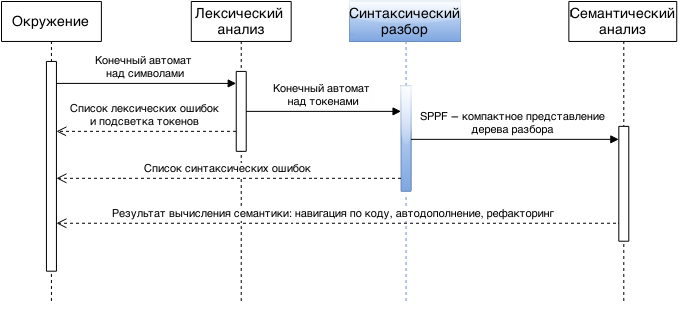
\includegraphics[width=15cm]{pics/Seq_rus.png}
 \caption{Диаграмма последовательности: взаимодействие компонентов
инструмента YaccConstructor}
 \label{seq}
\end{figure}

Предыдущая реализация платформы работала с грубой аппроксимацией, которая не осуществляла поддержку формирования выражения в циклах и с помощью строковых выражений~\cite{SECR13}. Используемая аппроксимация не являлась аппроксимацией сверху, что сказывалось на точности результатов анализа, и поэтому впоследствии она была заменена на регулярную. Однако это повлекло необходимость изменения алгоритма синтаксического анализа, чему и посвящена данная работа. 